\chapter{Introduction}
%
\section{Terms and Definitions}
    \subsection*{Free Harmonic and Damped Oscillation}
        If a system capable of oscillation is deflected out of its equilibrium position and is experiencing a restoring force
        proportional to its deflection this system is called a \textit{harmonic oscillator}. If a dampening force such as friction
        is introduced, the system no longer oscillates freely but rather damped.\par
        Both, damped and harmonic oscillations are considered \textit{free} if there is no continuous, the oscillation driving
        stimulus present.
        %
    \subsection*{Natural Angular Frequency of a Harmonic Oscillation}
        %
        Depending on the very characteristics of the given system it will oscillate at a distinct frequency - the natural angular
        frequency \( \omega_0 \).
    \subsection*{Differential Equation of the Damped Harmonic Oscillation}
        \begin{equation}
            J \ddot{\varphi} = -D\varphi -\rho\dot{\varphi}+M\cos(\omega t) \footnote{\textcite{Eichler.2016}}
        \end{equation}
    \subsection*{Damping cases}
        Overdamped: The system returns to equilibrium without oscillating.\par
        Critically damped: The system returns to equilibrium as quickly as possible without oscillating.\par
        Underdamped: The system oscillates (at reduced frequency compared to the undamped case) with the amplitude gradually
        decreasing to zero.
    \subsection*{Rotational Inerta}
        A cylindrical rod has a rotational inertia about its center of: \(J_S = \frac{1}{12}ml^2\)
        %
    \subsection*{\textsc{Steiner}'s Theorem}
        \textsc{Steiner}'s Theorem: \(J = J_S + mr^2\)
        %
    \subsection*{Eddy Current Brake}
        The equivalent circuit of a conductor exposed to a changing magnetic field is composed of only a voltage source
        and a resistor. The voltage across this resistor is induced as of the law of electromagnetic induction: \(U_{ind} = -NA\frac{\partial B}{\partial t}\).
        The resulting current creates a magnetic field opposing the inducing field. If the change of the inducing magnetic
        field is due to a mechanical movement, the induced magnetic field will this movement as well.
        % Eddy currents are created when a conductor passes through a magnetic field, which creates opposing forces that spin
        % inside the conductor. According to Lenz’s law, an eddy current produces a magnetic field that is in opposition
        % to the magnetic field that produced it, and therefore eddy currents are an inverse response to the source magnetic field.
        %
    \subsection*{Constant Current Constant Voltage Operation of a PSU}
        As the name implies a power supply in CC/CV (\textbf{C}onstant \textbf{C}urrent/\textbf{C}onstant \textbf{V}oltage)
        operation mode keeps the output current and/or output voltage constant independently of the load applied.
        % In constant voltage mode, which is sometimes referred to as voltage-controlled mode, a power supply behaves like
        % a voltage source, holding the voltage across the output terminals constant while the current output varies,
        % depending on load conditions. Constant current mode is essentially the opposite of constant voltage mode. In
        % constant current mode, also known as current-controlled mode, the power supply behaves like a current source,
        % holding the current flowing through the output terminals constant while the output voltage varies depending on
        % load conditions.
        %
    \subsection*{Capacitance of a Parallel Plate Capacitor}\label{sec:capacitance of a parallel plate capacitor}
        The capacitance of a parallel plate capacitor is: \(C = \varepsilon_0 \varepsilon_r \cdot \frac{A}{d}\)
        %
    \subsection*{Time-Constant of an RC-Circuit}
        The time constant of an RC circuit: \(\tau = RC\)
    %
\section{Preparation}
%
    \subsection{Deriving the Equation for Damped Free Oscillation}\label{sec:preparation_task_1}
    %
        \begin{equation}
            \vec{M}_{ Inert } + \vec{M}_{ Frict } + \vec{ M}_{ Rest } = 0 \quad \Leftrightarrow \quad J \cdot \ddot\varphi(t) - k \cdot \dot\varphi(t) - D^* \cdot \varphi(t) = 0
        \end{equation}
        can be written as
        \begin{equation}
            \ddot\varphi(t) + 2 \delta \cdot \dot\varphi(t) + \omega_0^2 \cdot \varphi(t) = 0
            \label{eq:dampedOscillation}
        \end{equation}
        with
        \begin{equation}
            -\frac{k}{J} = 2\delta, \quad -\frac{D^*}{J} = \omega_0^2
            \label{eq:DEParameters}
        \end{equation}
        whereas \cref{eq:dampedOscillation} is a second degree harmonic differential equation.
        The chosen approach is:
        \begin{equation}
            \varphi(t) = \hat{\varphi} e^{\lambda t}, \quad \dot{\varphi}(t) = \lambda \hat{\varphi} e^{\lambda t}, \quad \ddot{\varphi}(t) = \lambda^2 \hat{\varphi} e^{\lambda t}
        \end{equation}
        Plugged into \cref{eq:dampedOscillation} gives
        \begin{align}
            \left(\lambda^2 + 2\delta \lambda + \omega_0^2\right) \hat{\varphi}e^{\lambda t} = 0 \nonumber \\
            \lambda_{1,2} = -\delta \pm \sqrt{\delta^2-\omega_0^2} \nonumber \\
        \end{align}
        Here two possible cases are to be distinguished:
        \begin{equation}
            \lambda_{1,2} =
            \begin{cases}
                    -\delta \pm i\omega_d \qquad \text{for} \qquad \delta^2 < \omega_0^2 \quad \text{(a)}\\
                    -\delta \pm \omega_d \qquad \text{for} \qquad \delta^2 \geq \omega_0^2 \quad \text{(b)}
            \end{cases}
        \end{equation}
        In \cref{eq:dampedOscillation}:
        \begin{equation}
            \varphi_1(t) = \varphi_1 e^{-\delta + i\omega_d t}, \quad \varphi_2(t) = \varphi_2 e^{-\delta - i\omega_d t}
        \end{equation}
        Linear combination of \( \varphi_1(t) \) and \( \varphi_2(t) \) lastly leads to
        \begin{equation}
            \varphi(t) = \varphi_1 e^{-\delta + i\omega_d t} + \varphi_2 e^{-\delta - i\omega_d t} = \hat{\varphi}e^{-\delta t} \cdot \cos{\left( \omega_d t + \varphi_0 \right)}
        \end{equation}
        %
    \subsection{Damping Cases}\label{sec:preparation_task_2}
    %
    \begin{figure}[H]
        \centering
        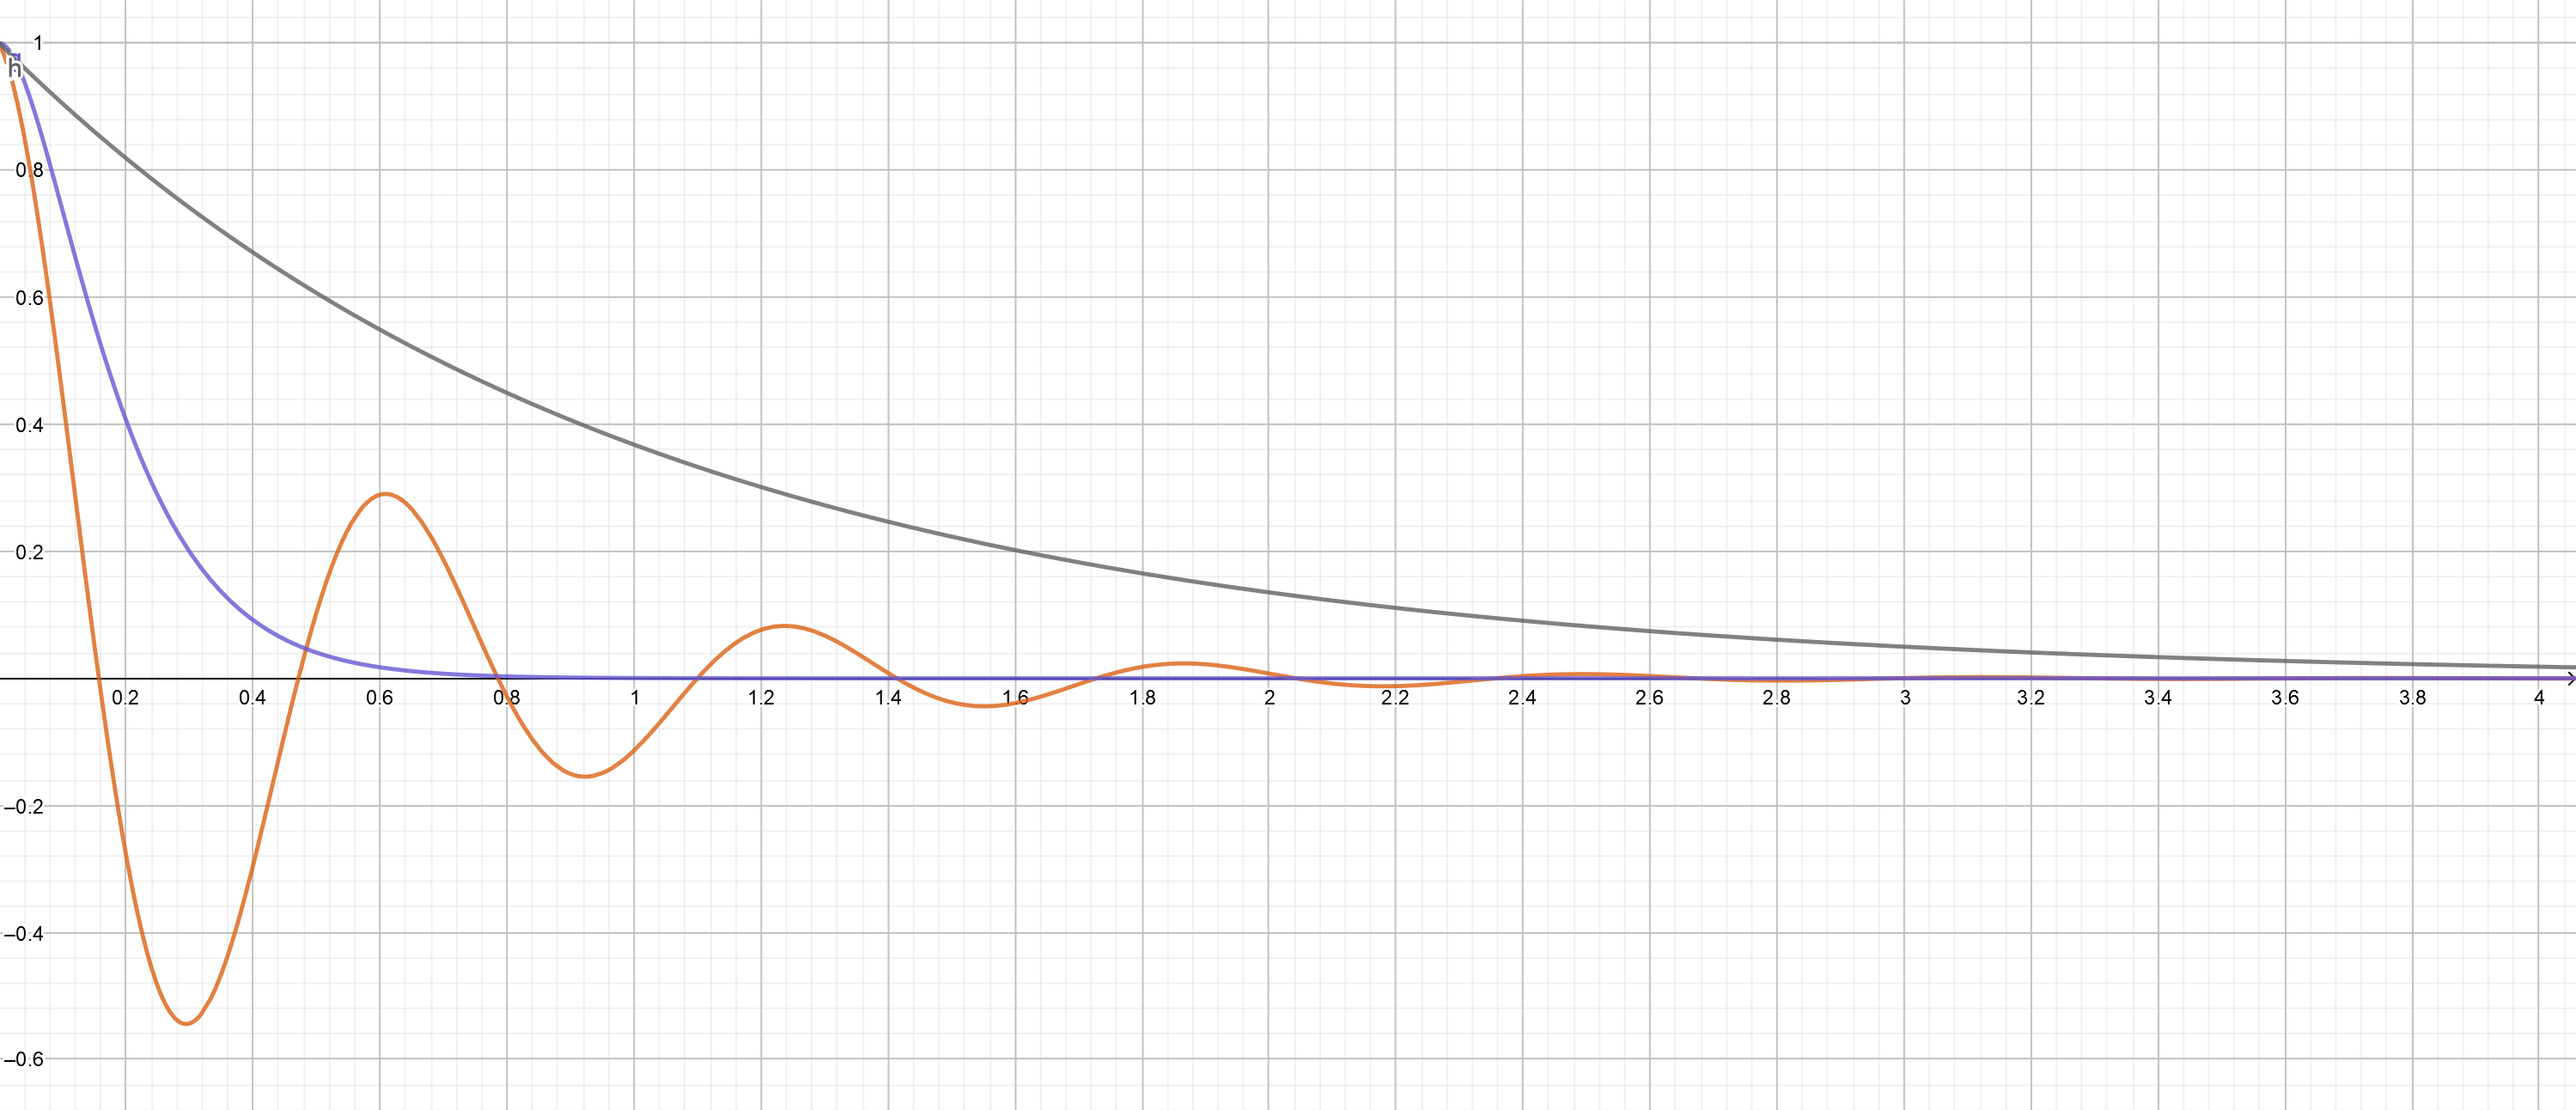
\includegraphics[width=.9\textwidth]{Preparation/damping_cases.png}
        \caption[Damping cases of a harmonic oscillation]{Plot of amplitude against time of a harmonic oscillation with
        parameterized damping coefficient. Orange: underdamped, Gray: overdamped, Blue: critically damped.}
        \label{fig:damping_cases_prepTask_2}
    \end{figure}
    %
    \subsection{Unknown Angular Inertia of the Pendulum}\label{sec:preparation_task_3}
    %
        The angular inertia of the pendulum \( J_P \) can be determined by adding a known angular inertia \( J_R \) of a cylindrical rod. As \cref{eq:DEParameters} delivers
        %
        \begin{equation}
            \omega_0=\sqrt{\frac{D^*}{J}}
        \end{equation}
        %
        and \( \omega=\frac{2\pi}{T} \), the following relation is given:
        %
        \begin{align}
            \omega_{0,P}=\sqrt{\frac{D^*}{J_P}}=\frac{2\pi}{T_P} \quad              &\Leftrightarrow \quad 2\pi=T_P\cdot\sqrt{\frac{D^*}{J_P}} \label{eq:omegaP} \\
            \omega_{0,P+R}=\sqrt{\frac{D^*}{J_P+J_R}}=\frac{2\pi}{T_{P+R}} \quad    &\Leftrightarrow \quad 2\pi=T_{P+R}\cdot\sqrt{\frac{D^*}{J_P+J_R}} \label{eq:omegaP+R}
        \end{align}
        %
        When \cref{eq:omegaP} and \cref{eq:omegaP+R} are equated:
        %
        \begin{align}
                                    &T_P\cdot\sqrt{\frac{D^*}{J_P}}=T_{P+R}\cdot\sqrt{\frac{D^*}{J_P+J_R}} \nonumber\\
            \Leftrightarrow \quad   &\left( \frac{T_{P+R}}{T_P} \right)^2 =\frac{J_P+J_R}{J_P}=1+\frac{J_R}{J_P} \nonumber\\
            \Leftrightarrow \quad   &\frac{J_R}{J_P}=\left( \frac{T_{P+R}}{T_P} \right)^2-1 \nonumber\\
            \Rightarrow \quad       &J_P=\frac{J_R}{\left( \frac{T_{P+R}}{T_P} \right)^2-1}
            \label{eq:inertia}
        \end{align}
        %
        The angular inertia of the pendulum can be calculated without knowing the torsion constant \( D^* \).
        %
    \subsection{Rotational Inertia of a Cylindrical Rod}\label{sec:preparation_task_4}
        %
        \begin{figure}[h]
            \centering
            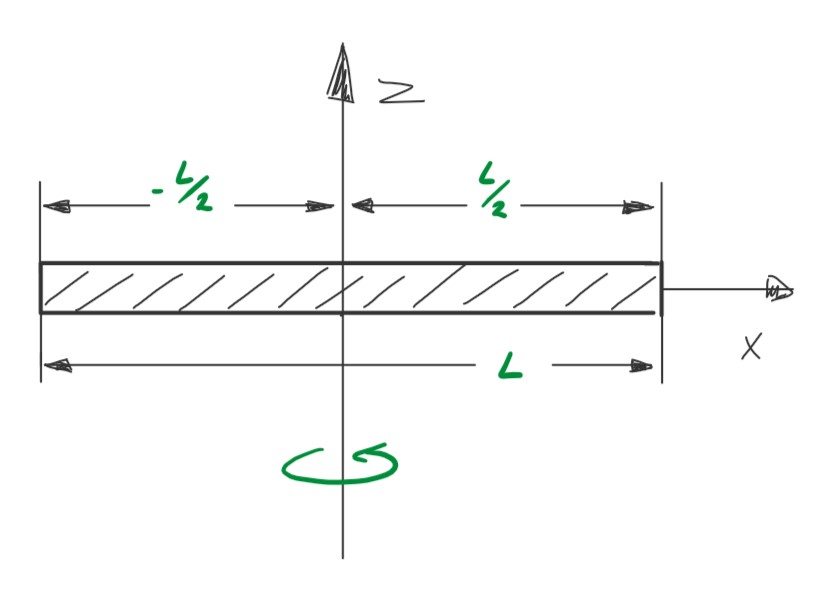
\includegraphics[width=.6\textwidth]{Preparation/rotating_rod.jpg}
            \caption[Rotating rod]{Scheme of a rod rotating orthogonally about its center axis.}
            \label{fig:rotationalIntertia_of_Cyl}
        \end{figure}
        %
        Inertia of a rotating dimensionless mass is proportional to the square of the distance to its rotational axis.
        As the mass of a cylindrical body is distributed over its volume, it is necessary to integrate over all \( dm  \) along
        the distance \( r \) from the center of rotation.
        \begin{equation}
            J_R = \int r^2 dm
            \label{eq:rotationalIntertia_of_Cyl}
        \end{equation}
        With
        \begin{equation}
            \rho = \frac{dm}{dx} = \frac{m}{L} \qquad \Leftrightarrow \qquad dm = \frac{m}{L} dx
        \end{equation}
        plugged into \cref{eq:rotationalIntertia_of_Cyl} with respect to the integration limits as of \cref{fig:rotationalIntertia_of_Cyl}
        gives
        \begin{equation}
            J_R = \int_{-\nicefrac{L}{2}}^{\nicefrac{L}{2}} \frac{m}{L} x^2 dx = \frac{1}{12}m L^2
            \label{eq:rotationalIntertia_of_Cyl alternate}
        \end{equation}
        %
    \subsection{Equations for the Sensor Capacitances}\label{sec:preparation_task_5}
        As described in \cref{sec:capacitance of a parallel plate capacitor}, the capacitance of a parallel plate capacitor
        is dependent on the overlapping area. Electrically, each vertical pair of capacitors are connected in parallel. They
        change there capacitance equally and in conjunction with the rotor rotating in any direction.\par
        % To derive:
        % \begin{align}
        %     C_1(\varphi) = \varepsilon_0 \frac{\pi D^2}{16 d} \left( 1 - \frac{2\varphi}{\pi} \right) \\
        %     \label{eq:capacitance 1 from tasks}
        %     C_2(\varphi) = \varepsilon_0 \frac{\pi D^2}{16 d} \left( 1 + \frac{2\varphi}{\pi} \right)
        %     \label{eq:capacitance 2 from tasks}
        % \end{align}
        % with
        % \begin{equation}
        %     A_{1,2}(\varphi) = \frac{1}{16}\pi D^2 \left( 1 \pm \frac{2\varphi}{\pi} \right)
        %     \label{eq:area from tasks}
        % \end{equation}
        %
        \begin{figure}[h]
            \centering
            \subfloat[Rotor at \( \varphi = \pm \frac{\pi}{2} \)\label{subfig:rotorAt pm halfPi}]{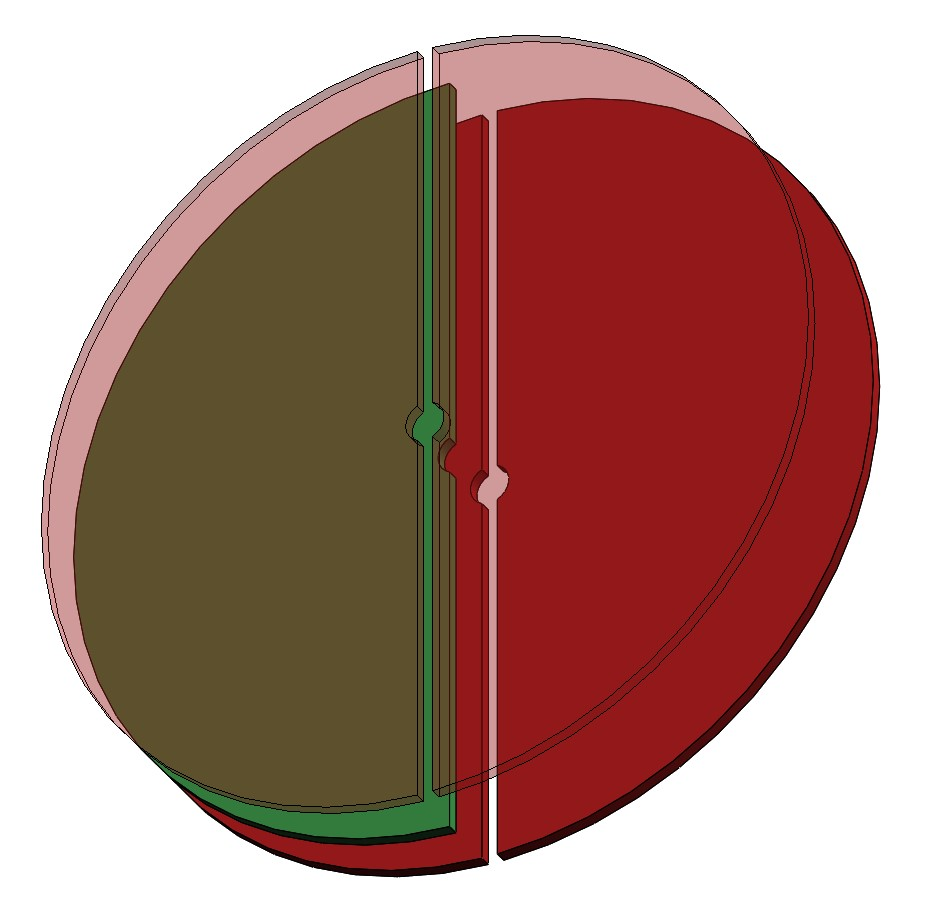
\includegraphics[width=.3\textwidth]{aufbau/statorRotorStator_pi.jpg}}
            \subfloat[Rotor at \( \varphi = 0 \)\label{subfig:rotorAt0}]{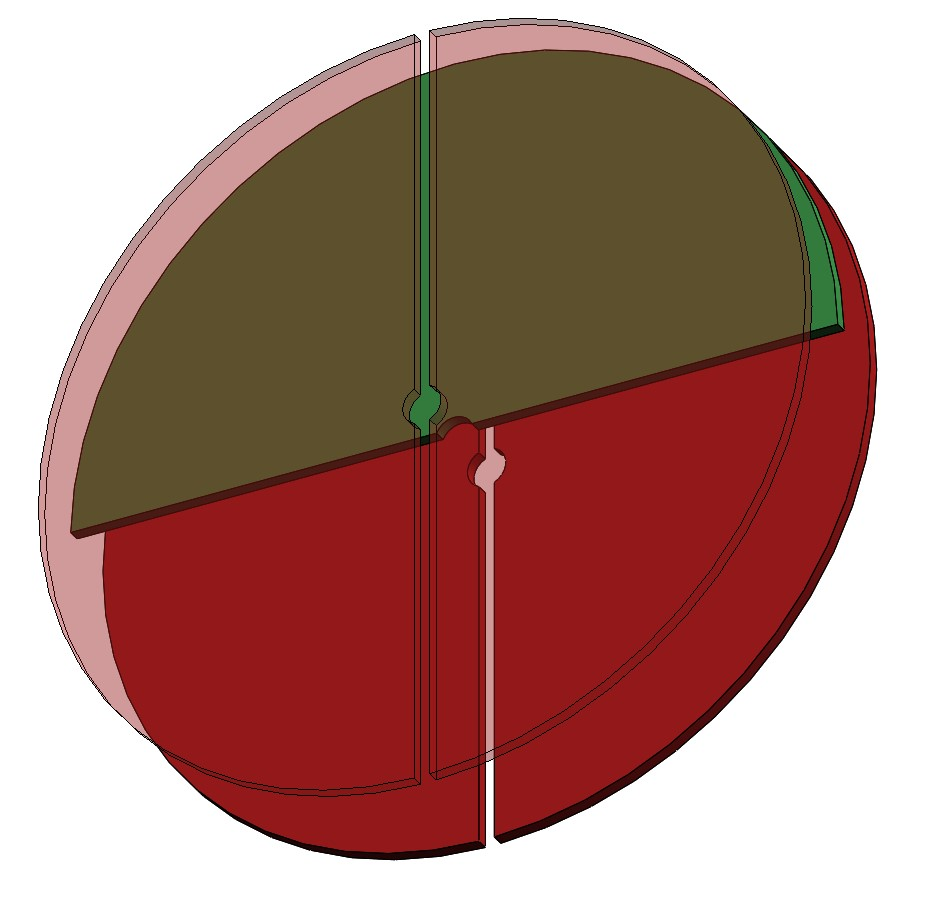
\includegraphics[width=.3\textwidth]{aufbau/statorRotorStator_0.5pi.jpg}}
            \subfloat[Rotor at \( \varphi = \mp \frac{\pi}{2} \)\label{subfig:rotorAt mp halfPi}]{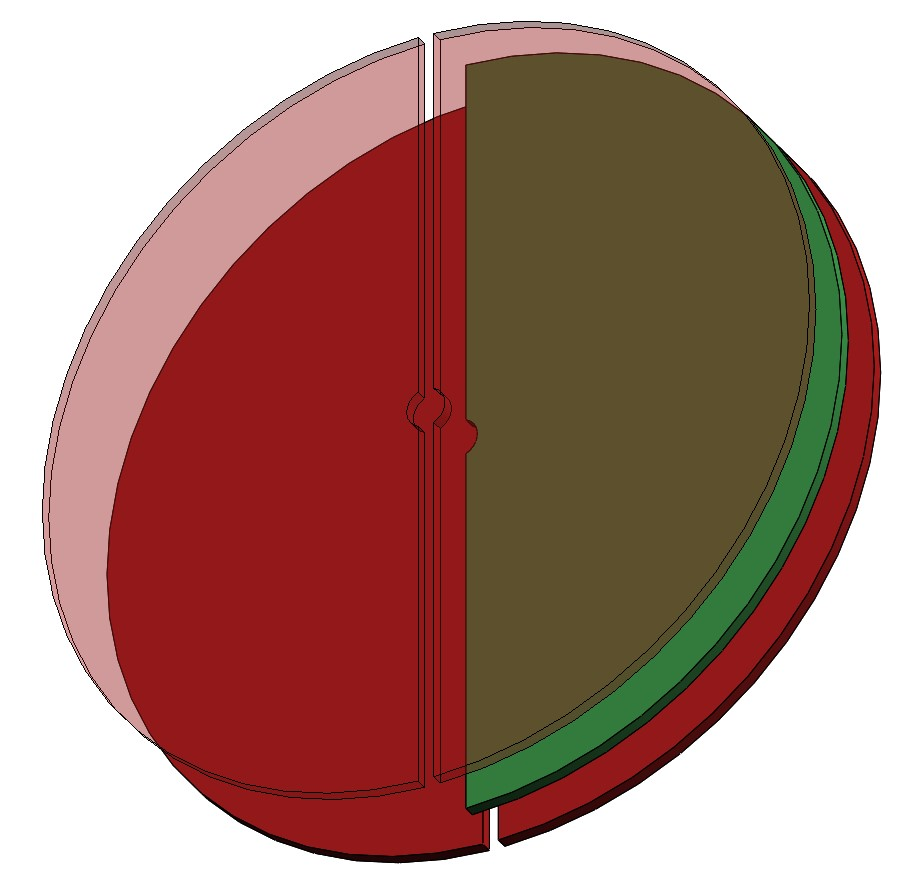
\includegraphics[width=.3\textwidth]{aufbau/statorRotorStator_0.jpg}}
            \caption[Schematic assembly of the angular sensor]{Schematic assembly of the angular sensor. The semi circular rotor plate (green) sandwiched between the two stators (red). The area of the rotor facing one of the vertical stator
            pairs varies with the angular displacement \( \varphi \)
            of the rotor.}
            \label{fig:rotorPositions}
        \end{figure}
        %
        Each of the vertically superimposed stator pairs together with the rotor plate form two capacitors connected in parallel
        with each capacitor having the same absolute value at any time. The total capacitance equates to
        \begin{equation}
            C_{1,2}(\varphi) = \varepsilon_0 \varepsilon_r \frac{A_{1,2}(\pm \varphi)}{d}
            \label{eq:angularCapacitance}
        \end{equation}
        Where \( A_{1,2}(\pm \varphi) \) can be expressed as
        \begin{align}
            A_{1,2}(\varphi)  &= \frac{1}{16}D^2 \left( \pi \pm 2\varphi \right) \nonumber \\
                        &= \frac{1}{16}D^2 \left( \frac{\pi^2}{\pi} \pm \frac{\pi}{\pi}2\varphi \right) \nonumber \\
                        &= \frac{1}{16} \pi D^2 \left( 1 \pm \frac{2\varphi}{\pi}\right)
            \label{eq:angularDependencyOfTheArea}
        \end{align}
        Say the zero-position is chosen such as each half of the rotor contributes to each of the stator pairs (see \cref{subfig:rotorAt0})
        \(A_1 = A_2\) applies. In any other case either \(A_1\) or \(A_2\) maximizes or minimizes respectively as shown in
        \cref{eq:rotation cases} (see \cref{subfig:rotorAt pm halfPi} and \cref{subfig:rotorAt mp halfPi} for reference).\par\medskip
        %
        Combining \cref{eq:angularCapacitance} and \cref{eq:angularDependencyOfTheArea} with \(\varepsilon_r = 1\) (air) gives
        %
        \begin{equation}
            C_{1,2} = \varepsilon_0 \frac{\pi D^2}{16d} \left( 1 \pm \frac{2\varphi}{\pi} \right) \quad \text{where} \quad \left(1 \pm \frac{2\varphi}{\pi} \right)
            \begin{cases}
                = 0 \quad \text{for} \quad \varphi = \mp \frac{\pi}{2} \nonumber \\
                = 1 \quad \text{for} \quad \varphi = 0 \nonumber \\
                = 2 \quad \text{for} \quad \varphi = \pm \frac{\pi}{2} \nonumber
            \end{cases}
            \label{eq:rotation cases}
        \end{equation}
        %
    \subsection{Time to Reach the Threshold Voltage}\label{sec:preparation_task_6}
        %
        The charging curve of a capacitor is given by \cref{eq:chargingCurve}.
        \begin{equation}
            U_C(t) = U_0 \left(1-exp\left(-\frac{t}{\tau}\right)\right)
            \label{eq:chargingCurve}
        \end{equation}
        Being interested at the time \( t_{th} \) it takes to reach a certain threshold voltage \( U_{th} \), \cref{eq:chargingCurve}
        can be transformed as follows:
        \begin{gather}
            1- \frac{U_{th}}{U_0} = exp\left(-\frac{t_{th}}{\tau}\right) \nonumber \\
            \Leftrightarrow \nonumber \\
            t_{th} = - \ln\left(1- \frac{U_{th}}{U_0}\right) \cdot \tau
            \label{eq:timeToThresholfVoltage}
        \end{gather}
        with the time constant \( \tau = R \cdot C \).
        %
    \subsection{Determining the Angular Deflection by the Difference of Timer Ticks}\label{sec:preparation_task_7}
        %
        The time to reach the threshold voltage as of \cref{eq:timeToThresholfVoltage} is captured independently due to
        each capacitor being connected to individual GPIOs.\par
        Since the charging curve of the capacitors differs in an anti-proportional manner when an angular deflection takes
        place the absolute value of the time difference gives the angle about zero while the sign gives the direction.
        Therefore, taken these considerations in account and merging \cref{eq:angularCapacitance} and \cref{eq:timeToThresholfVoltage}
        gives:
        \begin{align}
            \Delta t_{th}(\varphi)   &= t_{th,1} - t_{th,2} = -\ln\left( 1- \frac{U_{th}}{U_0} \right)R\left[ C_1(\varphi) - C_2(\varphi) \right] \nonumber \\
                            &= -\varepsilon_0 R \frac{\pi D^2}{16d} \ln\left( 1 - \frac{U_{th}}{U_0} \right) \left[ \left( 1 + \frac{2\varphi}{\pi} \right) - \left( 1 - \frac{2\varphi}{\pi} \right) \right] \nonumber \\
                            &= -\varepsilon_0 R \frac{4D^2}{16d} \ln\left( 1 - \frac{U_{th}}{U_0} \right) \cdot \varphi
            \label{eq:time_to_reach_thresholdVoltage}
        \end{align}
        Here \( \varepsilon_0 \), \( R \), \( D \), \( d \), \( U_{th} \) and \( U_0 \) remain constant and can be gathered as a proportionality
        factor. This reduces \cref{eq:time_to_reach_thresholdVoltage} to
        \begin{equation}
            \Delta t_{th}(\varphi) = \chi \cdot \varphi
            \label{eq:simplified_time_to_reach_thresholdVoltage}
        \end{equation}
        The \micro C checks the state of the input pin once every cycle. To take that into account the difference in threshold time
        \( \Delta t_{th} \) has to be divided by the cycle time \( \Delta t \) of the \micro C which gives the number of cycles it took for the
        input pins to switch state from low to high. If a change takes place at a non integer multiple of \( \Delta t \)
        the \micro C will register a transition on the subsequent cycle, thus, for the cycle count \( n \) applies \( n \in \mathbb{N} \).
        Furthermore, a non-integer value for \( n \) has to be rounded up to the next integer value.

        Mathematically the above considerations yield
        \begin{equation}
            n(\varphi) = \left\lceil \frac{\left\vert \Delta t_{th}(\varphi) \right\vert }{\Delta t} \right\rceil = \left\lceil \chi' \cdot \vert\varphi\vert \right\rceil \qquad \text{with} \qquad n(\varphi): n(\varphi) \in \mathbb{N}
            \label{eq:value_of_cycle_Count}
        \end{equation}
        which translates into the amount of deflection and
        \begin{equation}
            \frac{\vert n(\varphi)\vert}{n(\varphi)} = \pm 1
            \label{eq:sign_of_cycle_count}
        \end{equation}
        to distinguish between a CW/CCW rotation.
        %
    \subsection{Sensitivity of the Angular Sensor}\label{sec:preparation_task_8}
        %
        As seen in \cref{eq:simplified_time_to_reach_thresholdVoltage}, the tick rate relates linearly with the angular displacement \( \varphi \).
        Therefore, the maximum resolution of the angular sensor expressed as \textit{ticks per radiant} is \( \chi' \).
        \begin{equation}
            \frac{dn(\varphi)}{d\varphi} = \chi' \cdot \varphi \frac{d}{d\varphi} = \chi'
        \end{equation}
        \begin{figure}[H]
            \centering
            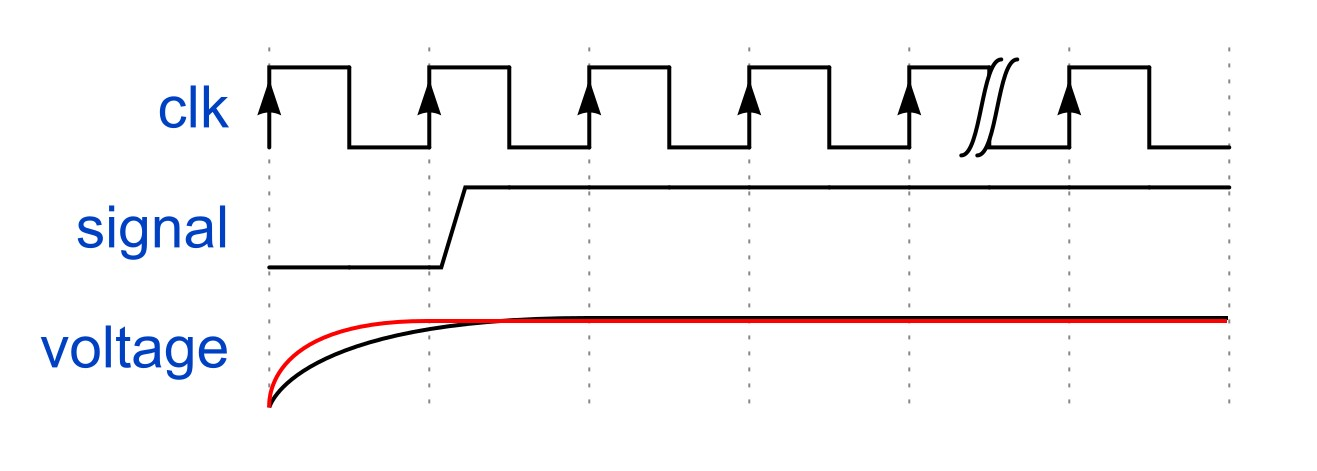
\includegraphics[width=.7\textwidth]{aufbau/clk_signal_timing_diagram.jpg}
            \caption[Timing diagram showing the signal transition]{Timing diagram showing the signal transition.}
            \label{fig:timing_diagram}
        \end{figure}
        The clock frequency of the \micro C is \( f = \SI{16}{MHz} \) which gives a cycle time of \( \Delta t = \SI{62.5}{ns} \).
        
        To ready the capacitors for the next charging cycle they need to be discharged as quick as possible. Considering
        that a time to discharge the capacitors \( < \Delta t \) makes no significant difference the unknown value \( R \)
        of the resistor can be approximated as
        \begin{gather}
            3\tau = \Delta t = 3RC \nonumber \\
            \Leftrightarrow \nonumber \\
            \frac{\Delta t}{3C_{max}} = R
            \label{eq:resistor_approximation}
        \end{gather}
        In the equation above the assumptions are made that a discharge rate of 95\% is sufficient and the circuit needs
        to be able to discharge the capacitor within the timeframe \( \Delta t \) while being at its maximum capacitance.
        Thus,
        \begin{align}
            C_{max} &= \varepsilon_0 \frac{\pi D^2}{8d} \nonumber \\
                    &= \SI{8,85\cdot10^{-12}}{\frac{\ampere\second}{\volt\metre}} \frac{\pi \cdot \SI{0.12^2}{m^2}}{8 \cdot \SI{0.01}{m}} \nonumber \\
                    &= \SI{5.01}{pF}
            \label{val:C_max}
        \end{align}
        in \cref{eq:resistor_approximation} gives a value for the resistance as
        \begin{equation}
            \frac{\SI{62.5}{ns}}{3 \cdot \SI{5.01}{pF}} \approx \SI{4160.9}{k\ohm}
        \end{equation}
        This lies between the two more common E-Series values of \(\SI{4.7}{k\ohm}\) and \(\SI{3.9}{k\ohm}\). For further calculations
        the latter is chosen as a higher resistance would increase the discharge time.\par\medskip
        Plugging in the given values of for \( \varepsilon_0, D, d, U_{th}, U_0 \) and the calculated values for \( \Delta t \text{ and } R \)
        equates \cref{eq:simplified_time_to_reach_thresholdVoltage} to
    
        \begin{align}
            \chi'   &= -\varepsilon_0 R \frac{4 D^2}{16d} \ln\left( 1 - \frac{U_{th}}{U_0} \right) \Delta t^{-1} \nonumber \\
                    &= -\SI{8.85 \cdot 10^{-12}}{\frac{As}{Vm}} \cdot \SI{3.9}{k\ohm} \cdot \frac{4 \cdot \SI{0.12^2}{\metre\squared}}{16 \cdot \SI{0.01}{\metre}} \ln\left( 1 - \frac{\SI{2.5}{\volt}}{\SI{5}{\volt}} \right) \cdot \frac{1}{\SI{62.5}{ns}} \nonumber \\
                    &\approx \SI{0.138}{\radian^{-1}}
                    \label{eq:est.sensitivity}
        \end{align}
        \nocite{Demtroder.2018.Experimentalphysik.1}\nocite{Eichler.2016}